%----------------------------------------------------------------------------------------
%	PACKAGES AND DOCUMENT CONFIGURATIONS
%----------------------------------------------------------------------------------------

\documentclass[12pt]{article}

\usepackage{graphicx} % Required for the inclusion of images
\usepackage[square,sort,comma,numbers]{natbib}
\usepackage{amsmath} % Required for some math elements 
\usepackage{import}
\usepackage[section]{placeins}

\usepackage{cmap}
\usepackage[T2A]{fontenc}
\usepackage[utf8x]{inputenc}
\usepackage[english, russian]{babel}
\usepackage[a4paper,left=15mm,right=15mm,top=30mm,bottom=20mm]{geometry}

\usepackage{xcolor}
\usepackage{hyperref}
\usepackage{adjustbox}

\usepackage{listings}
\lstset{language=R, basicstyle=\small, extendedchars=\true, breaklines=true, breakatwhitespace=true} 

\hypersetup{pdfstartview=FitH, linkcolor=black, urlcolor=black, citecolor=black, colorlinks=true}

\setlength\parindent{0pt} % Removes all indentation from paragraphs

\renewcommand{\labelenumi}{\arabic{enumi}.}

\addto\captionsrussian{\def\refname{Литература}}

% \sloppy
% \voffset=-20mm
% \textheight=235mm
% \hoffset=-25mm
% \textwidth=180mm
% \headsep=12pt
% \footskip=20pt


%----------------------------------------------------------------------------------------
%	DOCUMENT INFORMATION
%----------------------------------------------------------------------------------------
\begin{document}
\import{../}{titlepage.tex}

\tableofcontents
\clearpage

\listoffigures
\clearpage

\listoftables
\clearpage
 
%----------------------------------------------------------------------------------------
%	SECTION 1
%----------------------------------------------------------------------------------------

\section{Постановка задачи}
Для 5 распределений:
\begin{itemize}
    \item Нормальное распределение $N(x,0,1)$
    \item Распределение Коши $C(x,0,1)$
    \item Распределение Лапласа $L(x,0,\frac{1}{\sqrt{2}})$
    \item Распределение Пуассона $P(k,10)$
    \item Равномерное распределение $U(x,-\sqrt{3},\sqrt{3})$
\end{itemize}

Необходимо:
\begin{enumerate}
    \item Сгенерировать выборки размером 10, 100 и 1000 элементов
    \item Вычислить для каждой них статистические характеристики положения данных: \\ $\overline{x}, med x, z_R, z_Q, z_tr$
    \item Повторить данные вычисления 1000 раз для каждой выборки и найти среднее характеристик положения $E(z)=\overline{z}$ и вычислить оценку дисперсии $D(z)=\overline{z^2}-{\overline{z}}^2$
    \item Представить полученные результаты в виде таблиц
\end{enumerate}


\section{Теория}
\import{../}{theory.tex}



\section{Реализация}
Лабораторная выполнена на языке Python, с использованием библиотек numpy, scipy,
matplotlib


\section{Результаты}
\subsection{Гистограммы и график плотности вероятности}

\begin{figure}[!hbt]
  \centering
  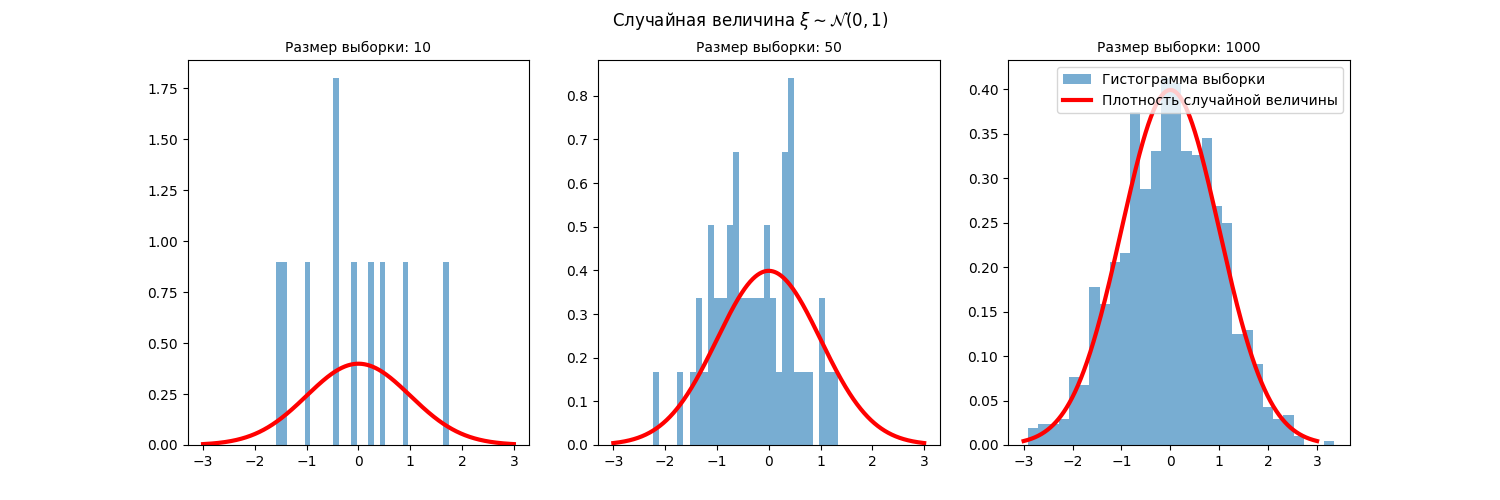
\includegraphics[width=0.8\paperwidth ]{images/histogram/normal.png}
  \centering
      \caption{Нормальное распределение}
\end{figure}

\begin{figure}[!hbt]
  \centering
  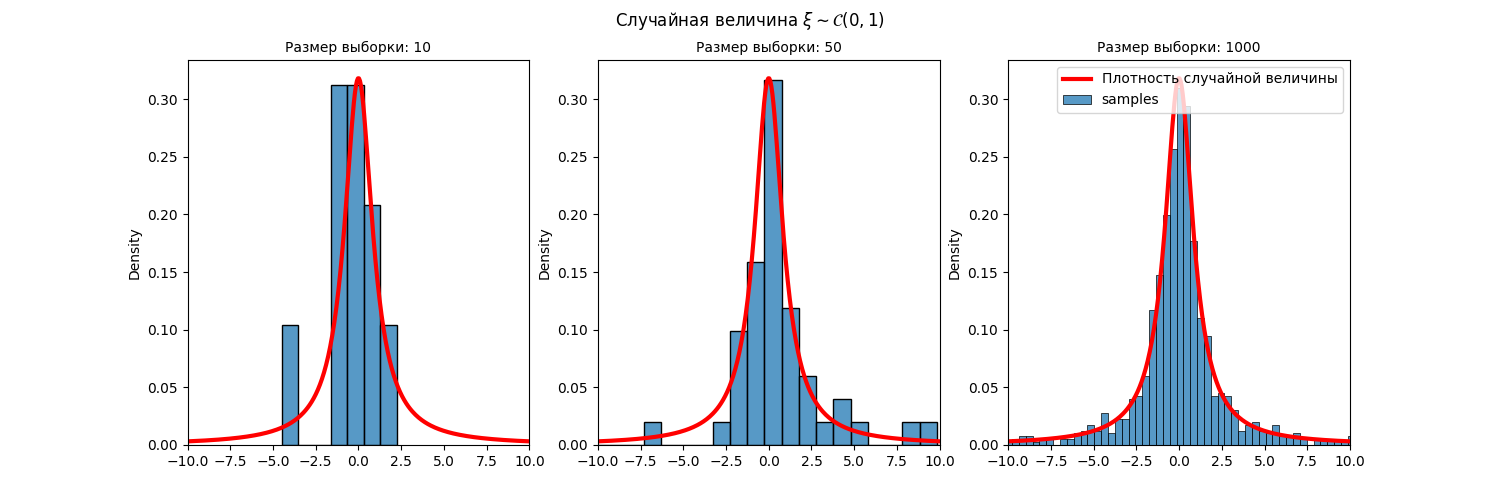
\includegraphics[width=0.8\paperwidth ]{images/histogram/cauchy.png}
  \caption{Распределение Коши}
\end{figure}

\begin{figure}[!hbt]
  \centering
  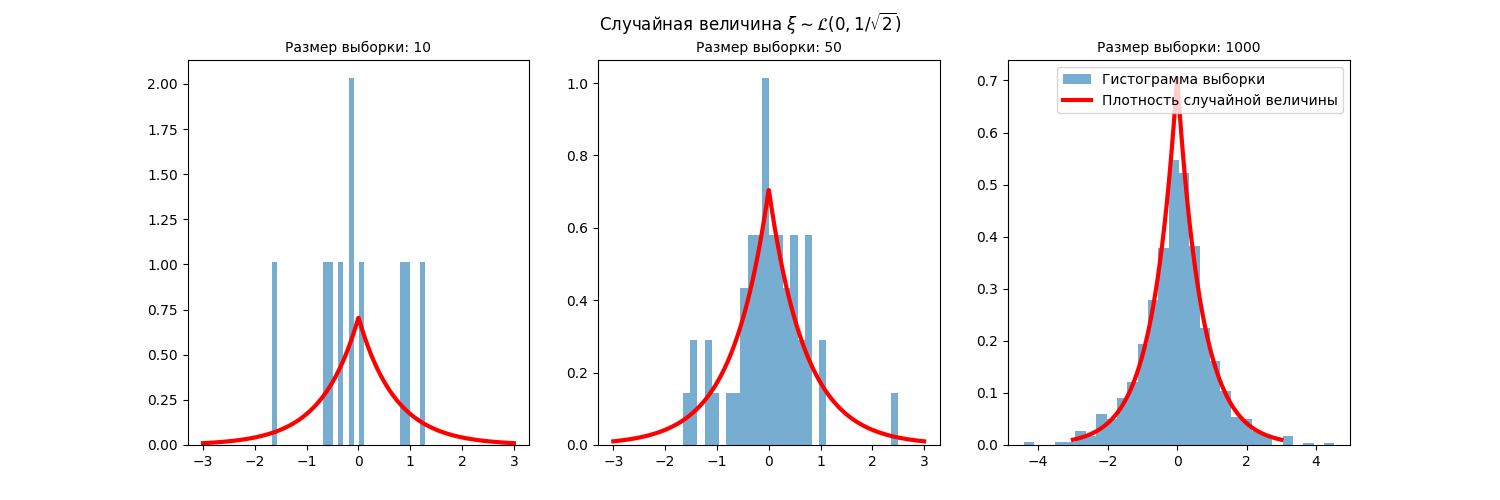
\includegraphics[width=0.8\paperwidth ]{images/histogram/laplace.png}
  \caption{Распределение Лапласа}
\end{figure}

\begin{figure}[!hbt]
  \centering
  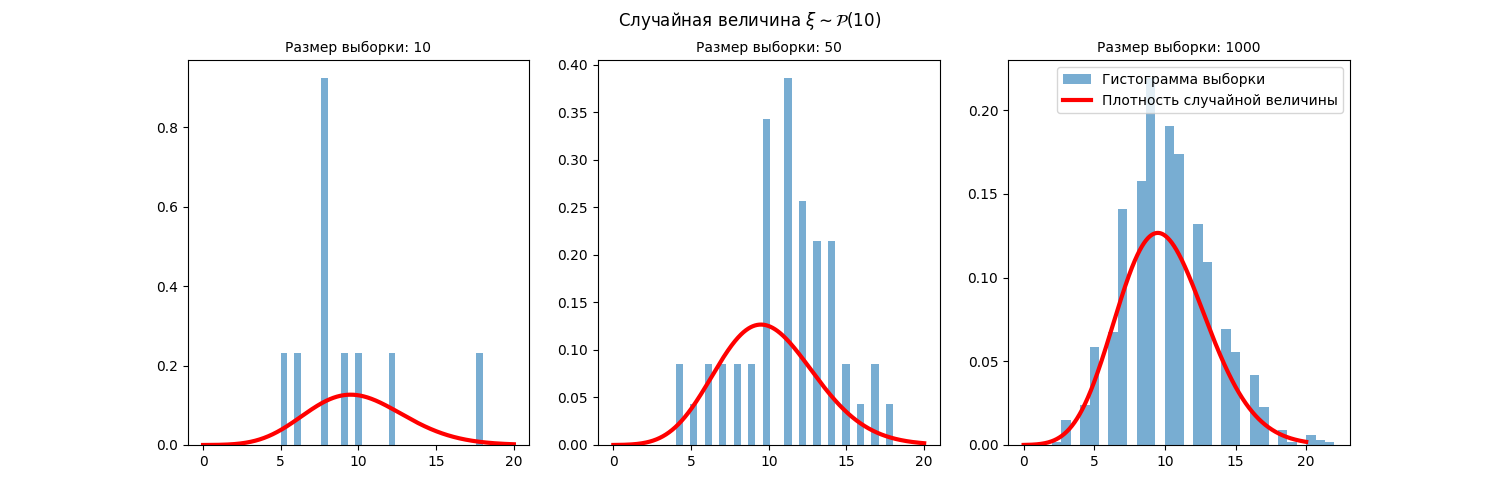
\includegraphics[width=0.8\paperwidth ]{images/histogram/poisson.png}
  \caption{Распределение Пуассона}
\end{figure}

\begin{figure}[!hbt]
  \centering
  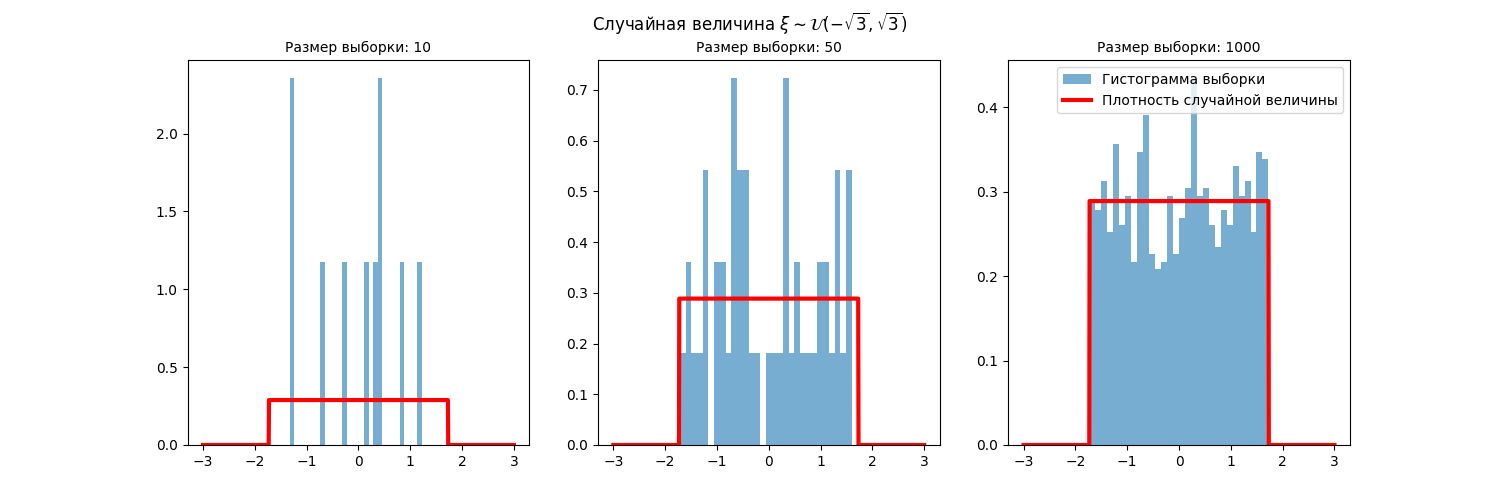
\includegraphics[width=0.8\paperwidth ]{images/histogram/uniform.png}
  \caption{Равномерное распределение}
\end{figure}

\FloatBarrier
\subsection{Характеристики положения и рассеяния}


\begin{center}
  \begin{table}[!hbt]
\caption{Нормальное распределение}
\begin{adjustbox}{width=\textwidth}
\begin{tabular}{| c | c | c | c | c | c |}
\hline
n = 10 & $\bar{x}$ & $med x$ & $z_R$ & $z_Q$ & $z_{tr}$ \\\hline
$E(z)$ & 0.0115 & 0.0105 & 0.0089 & 0.0124 & 0.0114 \\\hline
$D(z)$ & 0.0972 & 0.1335 & 0.1757 & 0.1103 & 0.1083 \\\hline
$E(z) \pm \sqrt{D(z)}$ & [-0.3003; 0.3233] & [-0.3548; 0.3759] & [-0.4102; 0.428] & [-0.3197; 0.3446] & [-0.3177; 0.3406]\\\hline
$\hat{E}(z)$ & 0 & 0 & 0 & 0 & 0 \\\hline
\end{tabular}
\end{adjustbox}

\begin{adjustbox}{width=\textwidth}
\begin{tabular}{| c | c | c | c | c | c |}
\hline
n = 100 & $\bar{x}$ & $med x$ & $z_R$ & $z_Q$ & $z_{tr}$ \\\hline
$E(z)$ & 0.0004 & 0.0021 & -0.0037 & -0.0024 & -0.0008 \\\hline
$D(z)$ & 0.0098 & 0.0153 & 0.0987 & 0.012 & 0.012 \\\hline
$E(z) \pm \sqrt{D(z)}$ & [-0.0987; 0.0994] & [-0.1215; 0.1257] & [-0.3179; 0.3105] & [-0.1118; 0.107] & [-0.1103; 0.1086]\\\hline
$\hat{E}(z)$ & 0 & 0 & 0 & 0 & 0 \\\hline
\end{tabular}
\end{adjustbox}

\begin{adjustbox}{width=\textwidth}
\begin{tabular}{| c | c | c | c | c | c |}
\hline
n = 1000 & $\bar{x}$ & $med x$ & $z_R$ & $z_Q$ & $z_{tr}$ \\\hline
$E(z)$ & 0.0013 & 0.0008 & 0.0027 & 0.0011 & 0.0009 \\\hline
$D(z)$ & 0.001 & 0.0016 & 0.0639 & 0.0012 & 0.0012 \\\hline
$E(z) \pm \sqrt{D(z)}$ & [-0.0306; 0.0331] & [-0.0391; 0.0408] & [-0.2501; 0.2555] & [-0.0341; 0.0362] & [-0.0338; 0.0356]\\\hline
$\hat{E}(z)$ & 0 & 0 & 0 & 0 & 0 \\\hline
\end{tabular}
\end{adjustbox}

\end{table}
\begin{table}[ht]
\caption{Распределение Коши}
\begin{adjustbox}{width=\textwidth}
\begin{tabular}{| c | c | c | c | c | c |}
\hline
n = 10 & $\bar{x}$ & $med x$ & $z_R$ & $z_Q$ & $z_{tr}$ \\\hline
$E(z)$ & 1.0513 & 0.0311 & 4.8835 & 0.0534 & 0.0412 \\\hline
$D(z)$ & 476.3827 & 0.3527 & 11518.0349 & 0.8528 & 0.5118 \\\hline
$E(z) \pm \sqrt{D(z)}$ & [-20.7749; 22.8775] & [-0.5628; 0.625] & [-102.4386; 112.2056] & [-0.8701; 0.9769] & [-0.6743; 0.7566]\\\hline
$\hat{E}(z)$ & - & 0 & - & 0 & 0 \\\hline
\end{tabular}
\end{adjustbox}

\begin{adjustbox}{width=\textwidth}
\begin{tabular}{| c | c | c | c | c | c |}
\hline
n = 100 & $\bar{x}$ & $med x$ & $z_R$ & $z_Q$ & $z_{tr}$ \\\hline
$E(z)$ & -2.5704 & -0.0017 & -127.1058 & 0.0081 & 0.0034 \\\hline
$D(z)$ & 3541.4148 & 0.0242 & 8826175.6291 & 0.0498 & 0.0256 \\\hline
$E(z) \pm \sqrt{D(z)}$ & [-62.0802; 56.9394] & [-0.1573; 0.154] & [-3097.9938; 2843.7823] & [-0.215; 0.2313] & [-0.1567; 0.1636]\\\hline
$\hat{E}(z)$ & - & 0 & - & 0 & 0 \\\hline
\end{tabular}
\end{adjustbox}

\begin{adjustbox}{width=\textwidth}
\begin{tabular}{| c | c | c | c | c | c |}
\hline
n = 1000 & $\bar{x}$ & $med x$ & $z_R$ & $z_Q$ & $z_{tr}$ \\\hline
$E(z)$ & 0.2454 & 0.0015 & 127.2055 & 0.0027 & 0.0018 \\\hline
$D(z)$ & 258.5488 & 0.0026 & 63214665.1176 & 0.0052 & 0.0027 \\\hline
$E(z) \pm \sqrt{D(z)}$ & [-15.8341; 16.3248] & [-0.0491; 0.0521] & [-7823.5596; 8077.9705] & [-0.0695; 0.0749] & [-0.0497; 0.0533]
\\\hline
$\hat{E}(z)$ & - & 0.0 & - & 0.0 & 0.0 \\\hline
\end{tabular}
\end{adjustbox}

\end{table}

\begin{table}
\caption{Распределение Лапласа}
\begin{adjustbox}{width=\textwidth}
\begin{tabular}{| c | c | c | c | c | c |}
\hline
n = 10 & $\bar{x}$ & $med x$ & $z_R$ & $z_Q$ & $z_{tr}$ \\\hline
$E(z)$ & -0.011 & -0.0144 & -0.0022 & -0.0108 & -0.0129 \\\hline
$D(z)$ & 0.0953 & 0.0731 & 0.3957 & 0.0833 & 0.0702 \\\hline
$E(z) \pm \sqrt{D(z)}$ & [-0.3196; 0.2976] & [-0.2847; 0.256] & [-0.6312; 0.6268] & [-0.2995; 0.2779] & [-0.278; 0.2521]\\\hline
$\hat{E}(z)$ & 0 & 0 & 0 & 0 & 0 \\\hline
\end{tabular}
\end{adjustbox}

\begin{adjustbox}{width=\textwidth}
\begin{tabular}{| c | c | c | c | c | c |}
\hline
n = 100 & $\bar{x}$ & $med x$ & $z_R$ & $z_Q$ & $z_{tr}$ \\\hline
$E(z)$ & 0.0027 & 0.0027 & -0.0136 & 0.0043 & 0.0033 \\\hline
$D(z)$ & 0.01 & 0.006 & 0.3971 & 0.0101 & 0.0065 \\\hline
$E(z) \pm \sqrt{D(z)}$ & [-0.0973; 0.1027] & [-0.0749; 0.0803] & [-0.6438; 0.6166] & [-0.0961; 0.1046] & [-0.0772; 0.0839]\\\hline
$\hat{E}(z)$ & 0 & 0.0 & 0 & 0 & 0.0 \\\hline
\end{tabular}
\end{adjustbox}

\begin{adjustbox}{width=\textwidth}
\begin{tabular}{| c | c | c | c | c | c |}
\hline
n = 1000 & $\bar{x}$ & $med x$ & $z_R$ & $z_Q$ & $z_{tr}$ \\\hline
$E(z)$ & 0.001 & 0.0014 & 0.0207 & 0.001 & 0.0011 \\\hline
$D(z)$ & 0.001 & 0.0005 & 0.3924 & 0.0011 & 0.0006 \\\hline
$E(z) \pm \sqrt{D(z)}$ & [-0.0307; 0.0326] & [-0.0215; 0.0243] & [-0.6057; 0.6471] & [-0.0315; 0.0336] & [-0.0238; 0.026]\\\hline
$\hat{E}(z)$ & 0.0 & 0.0 & 0 & 0.0 & 0.0 \\\hline
\end{tabular}
\end{adjustbox}

\end{table}

\begin{table}
\caption{Распределение Пуассона}
\begin{adjustbox}{width=\textwidth}
\begin{tabular}{| c | c | c | c | c | c |}
\hline
n = 10 & $\bar{x}$ & $med x$ & $z_R$ & $z_Q$ & $z_{tr}$ \\\hline
$E(z)$ & 10.0069 & 9.8435 & 10.3055 & 9.9328 & 9.8858 \\\hline
$D(z)$ & 1.0004 & 1.4263 & 1.9269 & 1.1702 & 1.1677 \\\hline
$E(z) \pm \sqrt{D(z)}$ & [9.0067; 11.0071] & [8.6492; 11.0378] & [8.9174; 11.6936] & [8.851; 11.0145] & [8.8052; 10.9664]\\\hline
$\hat{E}(z)$ & $ - $ & $ -  $ & $-$ & $-$ & $-$ \\\hline
\end{tabular}
\end{adjustbox}

\begin{adjustbox}{width=\textwidth}
\begin{tabular}{| c | c | c | c | c | c |}
\hline
n = 100 & $\bar{x}$ & $med x$ & $z_R$ & $z_Q$ & $z_{tr}$ \\\hline
$E(z)$ & 9.9988 & 9.8475 & 10.9135 & 9.9165 & 9.8568 \\\hline
$D(z)$ & 0.1026 & 0.232 & 0.9283 & 0.1472 & 0.1235 \\\hline
$E(z) \pm \sqrt{D(z)}$ & [9.6784; 10.3191] & [9.3658; 10.3292] & [9.95; 11.877] & [9.5329; 10.3001] & [9.5055; 10.2082]\\\hline
$\hat{E}(z)$ & $ - $ & $ -  $ & $-$ & $-$ & $-$ \\\hline
\end{tabular}
\end{adjustbox}

\begin{adjustbox}{width=\textwidth}
\begin{tabular}{| c | c | c | c | c | c |}
\hline
n = 1000 & $\bar{x}$ & $med x$ & $z_R$ & $z_Q$ & $z_{tr}$ \\\hline
$E(z)$ & 10.0055 & 9.998 & 11.655 & 9.997 & 9.8645 \\\hline
$D(z)$ & 0.0097 & 0.002 & 0.718 & 0.0028 & 0.0108 \\\hline
$E(z) \pm \sqrt{D(z)}$ & [9.907; 10.104] & [9.9533; 10.0427] & [10.8077; 12.5023] & [9.9438; 10.0502] & [9.7605; 9.9685]\\\hline
$\hat{E}(z)$ & $ - $ & $ -  $ & $-$ & $-$ & $9$ \\\hline
\end{tabular}
\end{adjustbox}

\end{table}

\begin{table}
\caption{Равномерное распределение}
\begin{adjustbox}{width=\textwidth}
\begin{tabular}{| c | c | c | c | c | c |}
\hline
n = 10 & $\bar{x}$ & $med x$ & $z_R$ & $z_Q$ & $z_{tr}$ \\\hline
$E(z)$ & 0.0018 & 0.0058 & -0.0063 & 0.0032 & 0.0044 \\\hline
$D(z)$ & 0.0995 & 0.225 & 0.0452 & 0.1398 & 0.1622 \\\hline
$E(z) \pm \sqrt{D(z)}$ & [-0.3137; 0.3172] & [-0.4686; 0.4802] & [-0.2189; 0.2063] & [-0.3707; 0.377] & [-0.3983; 0.4071]\\\hline
$\hat{E}(z)$ & $ 0 $ & $ 0 $ & $0$ & $0$ & $0$ \\\hline
\end{tabular}
\end{adjustbox}

\begin{adjustbox}{width=\textwidth}
\begin{tabular}{| c | c | c | c | c | c |}
\hline
n = 100 & $\bar{x}$ & $med x$ & $z_R$ & $z_Q$ & $z_{tr}$ \\\hline
$E(z)$ & 0.0034 & 0.0027 & -0.0003 & 0.0045 & 0.0041 \\\hline
$D(z)$ & 0.0105 & 0.0302 & 0.0005 & 0.0157 & 0.021 \\\hline
$E(z) \pm \sqrt{D(z)}$ & [-0.099; 0.1057] & [-0.1711; 0.1765] & [-0.0221; 0.0214] & [-0.1208; 0.1298] & [-0.1408; 0.1491]\\\hline
$\hat{E}(z)$ & $ 0.0 $ & $ 0 $ & $0.0$ & $0$ & $0$ \\\hline
\end{tabular}
\end{adjustbox}

\begin{adjustbox}{width=\textwidth}
\begin{tabular}{| c | c | c | c | c | c |}
\hline
n = 1000 & $\bar{x}$ & $med x$ & $z_R$ & $z_Q$ & $z_{tr}$ \\\hline
$E(z)$ & 0.0009 & 0.0011 & 0.0001 & 0.0008 & 0.0014 \\\hline
$D(z)$ & 0.001 & 0.003 & 0.0 & 0.0015 & 0.002 \\\hline
$E(z) \pm \sqrt{D(z)}$ & [-0.0308; 0.0325] & [-0.0536; 0.0558] & [-0.0023; 0.0025] & [-0.0386; 0.0401] & [-0.0435; 0.0463]\\\hline
$\hat{E}(z)$ & $ 0.0 $ & $ 0.0 $ & $0.00$ & $0.0$ & $0.0$ \\\hline
\end{tabular}
\end{adjustbox}

\end{table}
\end{center}

\FloatBarrier
\subsection{Боксплот Тьюки}
\begin{figure}[ht]
  \centering
  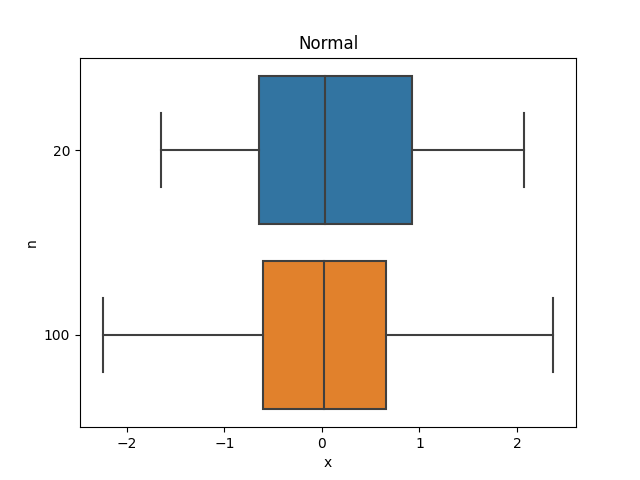
\includegraphics[width=0.4\paperwidth ]{images/boxplots/Normal.png}
  \caption{Нормальное распределение}
\end{figure}

\begin{figure}[ht]
  \centering
  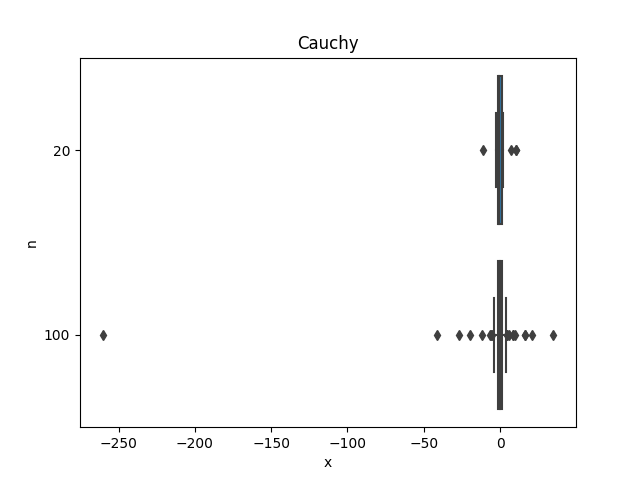
\includegraphics[width=0.4\paperwidth ]{images/boxplots/Cauchy.png}
  \caption{Распределение Коши}
\end{figure}

\begin{figure}
  \centering
  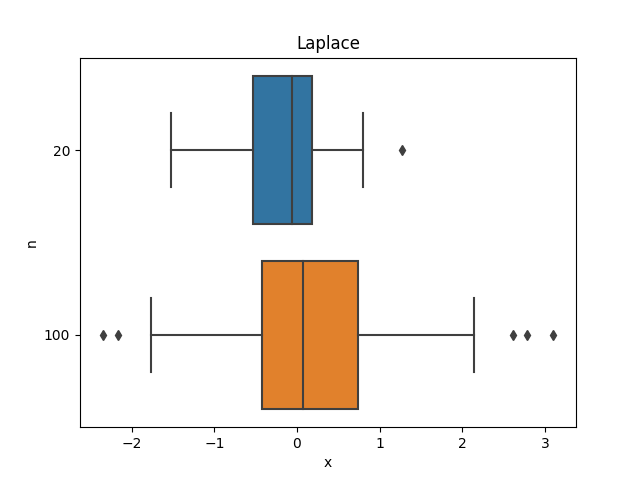
\includegraphics[width=0.4\paperwidth ]{images/boxplots/Laplace.png}
  \caption{Распределение Лапласа}
\end{figure}

\begin{figure}
  \centering
  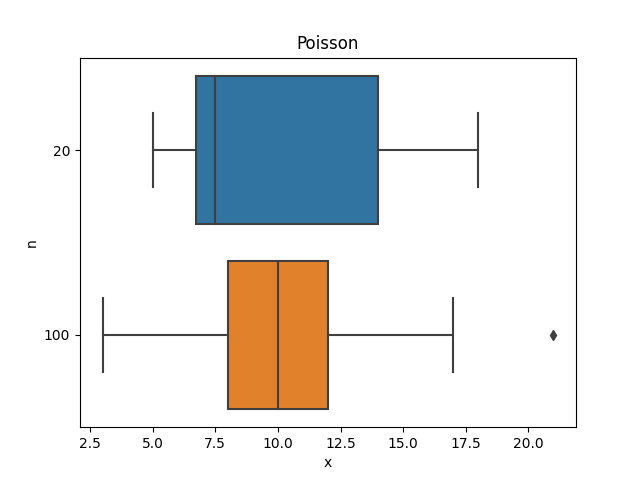
\includegraphics[width=0.4\paperwidth ]{images/boxplots/Poisson.png}
  \caption{Распределение Пуассона}
\end{figure}

\begin{figure}
  \centering
  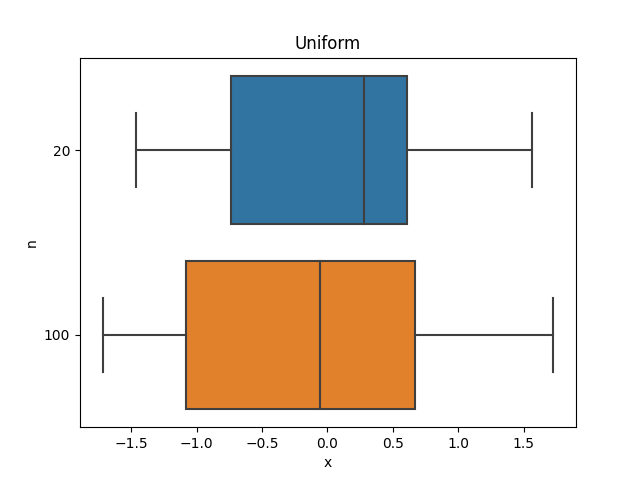
\includegraphics[width=0.4\paperwidth ]{images/boxplots/Uniform.png}
  \caption{Равномерное распределение}
\end{figure}

\FloatBarrier
\subsection{Доля выбросов}

\begin{table}[h!]
  \centering
  \begin{adjustbox}{width=0.5\textwidth}
    \begin{tabular}{| c | c | c |}

      \hline
      Распределение & n = 20 & n = 100 \\\hline
      Нормальное & 0.05 & 0.14 \\\hline
      Коши & 0.2 & 0.25 \\\hline
      Лапласа & 0.15 & 0.11 \\\hline
      Пуассона & 0.05 & 0.14 \\\hline
      Равномерное & 0.05 & 0.04 \\\hline
      
    \end{tabular}
  \end{adjustbox}
  \caption{Доля выбросов}
\end{table}


\FloatBarrier
\subsection{Теоретическая вероятность выбросов}
\begin{table}[h!]
  \centering
  \begin{adjustbox}{width=0.5\textwidth}
    \begin{tabular}{| c | c | c | c | c | c |}
      \hline
      Распределение & $Q^T_1$ & $Q^T_3$ & $X^T_1$ & $X^T_2$ & $P^T_B$ \\\hline
      Нормальное & -0.674 & 0.674 & -2.698 & 2.698 & 0.007 \\\hline
      Коши & -1 & 1 & -4 & 4 & 0.156 \\\hline
      Лапласа & -0.490 & 0.490 & -1.961 & 1.961 & 0.063 \\\hline
      Пуассона & 8 & 12 & 2 & 18 & 0.008 \\\hline
      Равномерное & -0.866 & 0.866 & -3.464 & 3.464 & 0 \\\hline
      
    \end{tabular}
  \end{adjustbox}
  \caption{Теоретическая вероятность выбросов}
\end{table}

\FloatBarrier
\subsection{Эмпирическая функция распределения}

\begin{figure}[h!]
  \centering
  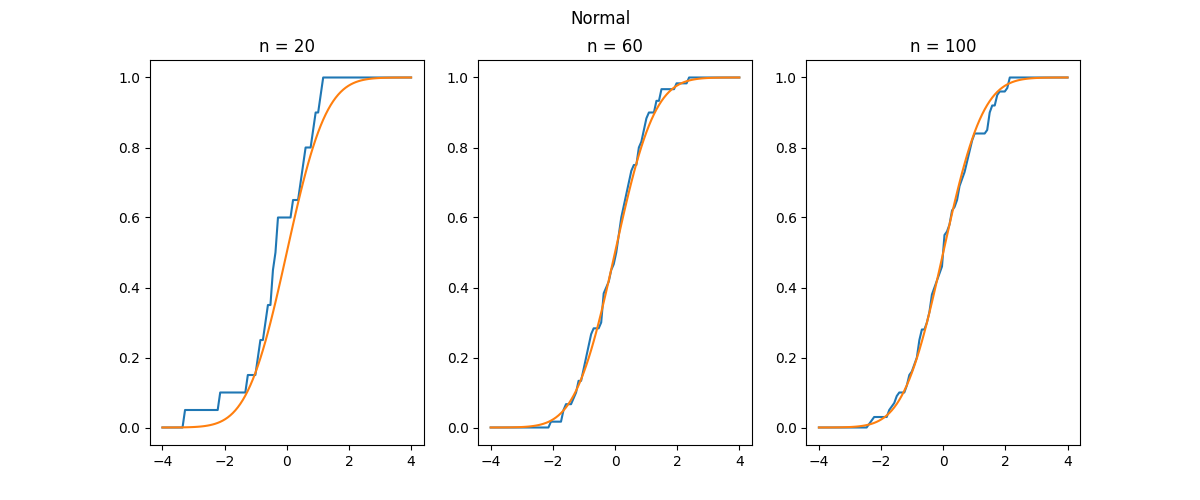
\includegraphics[width=0.8\paperwidth ]{images/edf/Normal.png}
  \caption{Нормальное распределение}
\end{figure}

\begin{figure}[h!]
  \centering
  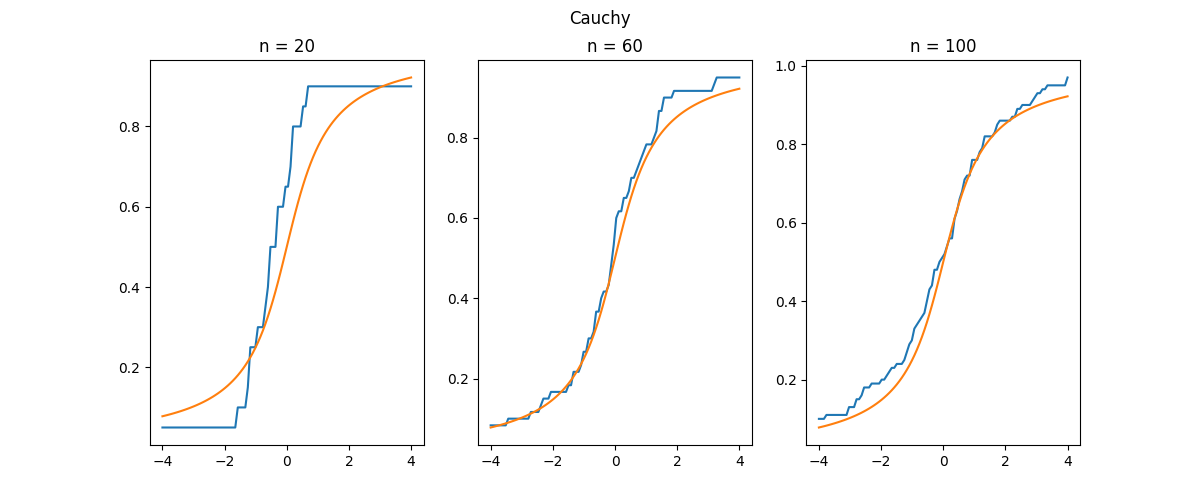
\includegraphics[width=0.8\paperwidth ]{images/edf/Cauchy.png}
  \caption{Распределение Коши}
\end{figure}

\begin{figure}[h!]
  \centering
  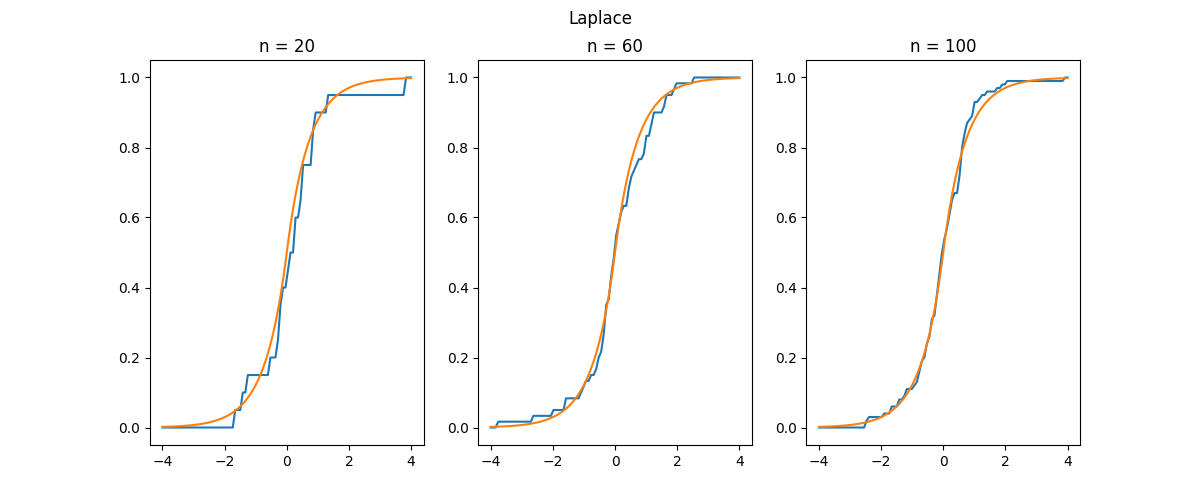
\includegraphics[width=0.8\paperwidth ]{images/edf/Laplace.png}
  \caption{Распределение Лапласа}
\end{figure}

\begin{figure}[h!]
  \centering
  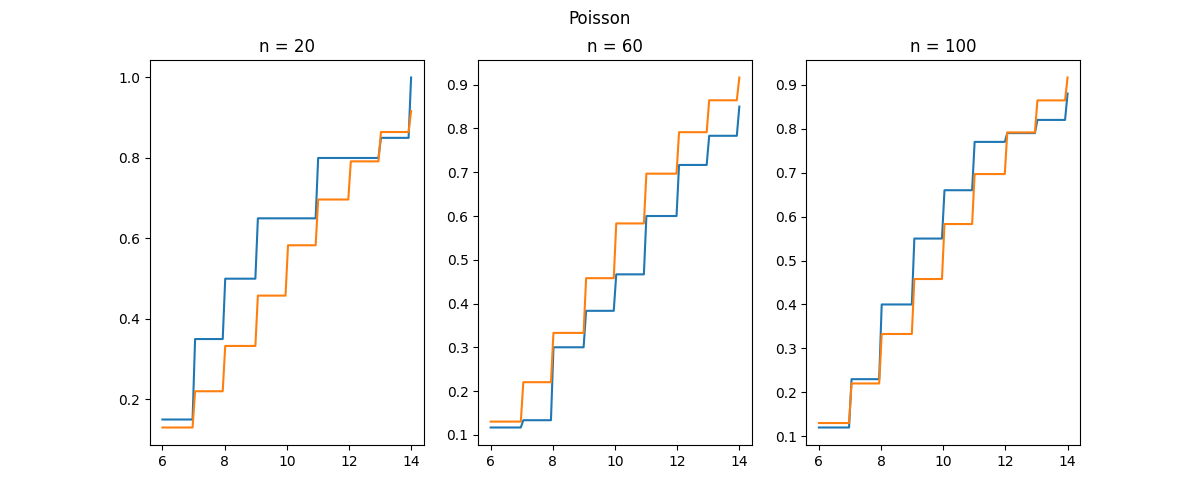
\includegraphics[width=0.8\paperwidth ]{images/edf/Poisson.png}
  \caption{Распределение Пуассона}
\end{figure}

\begin{figure}[h!]
  \centering
  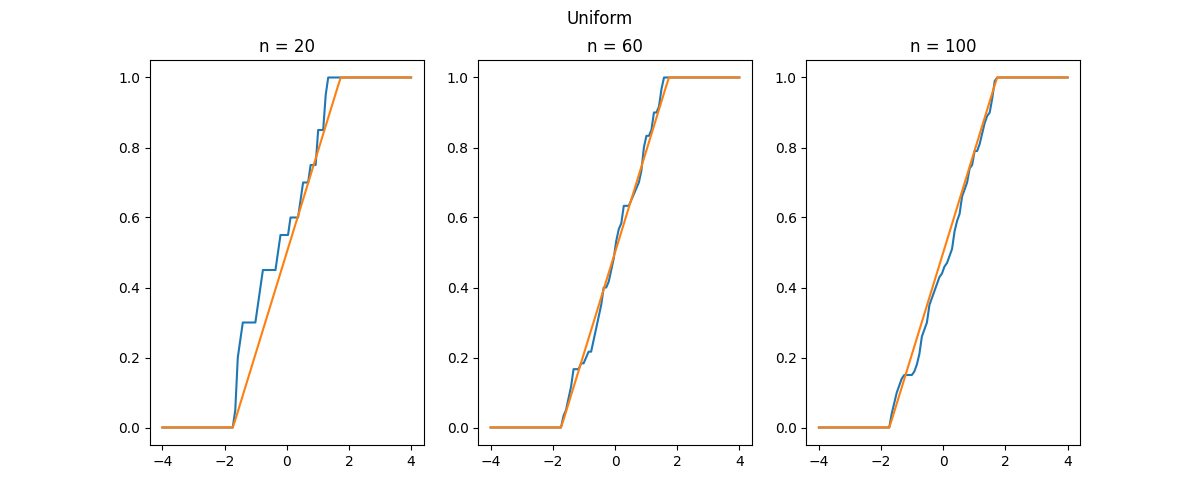
\includegraphics[width=0.8\paperwidth ]{images/edf/Uniform.png}
  \caption{Равномерное распределение}
\end{figure}

\FloatBarrier
\subsection{Ядерные оценки}
\begin{figure}[h!]
  \centering
  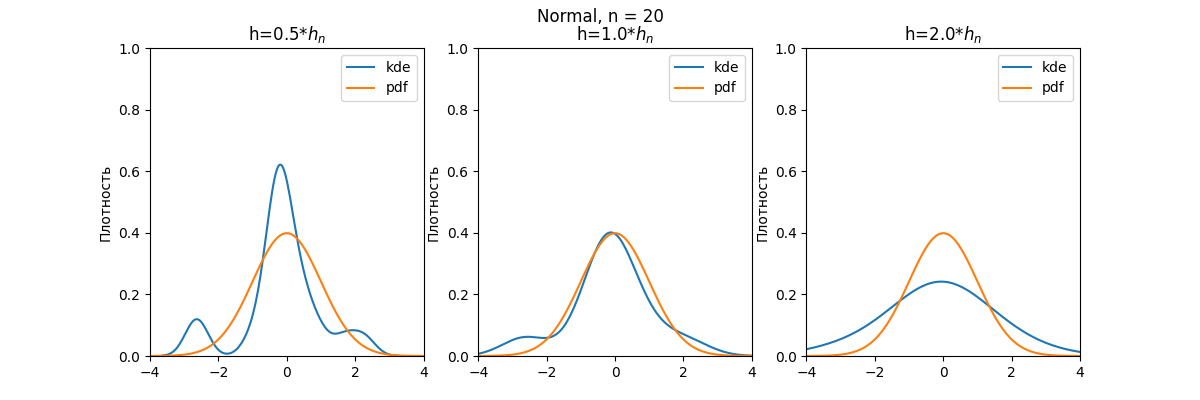
\includegraphics[width=0.8\paperwidth ]{images/kde/Normal_20.png}
  \caption{Нормальное распределение, n = 20}
\end{figure}

\begin{figure}[h!]
  \centering
  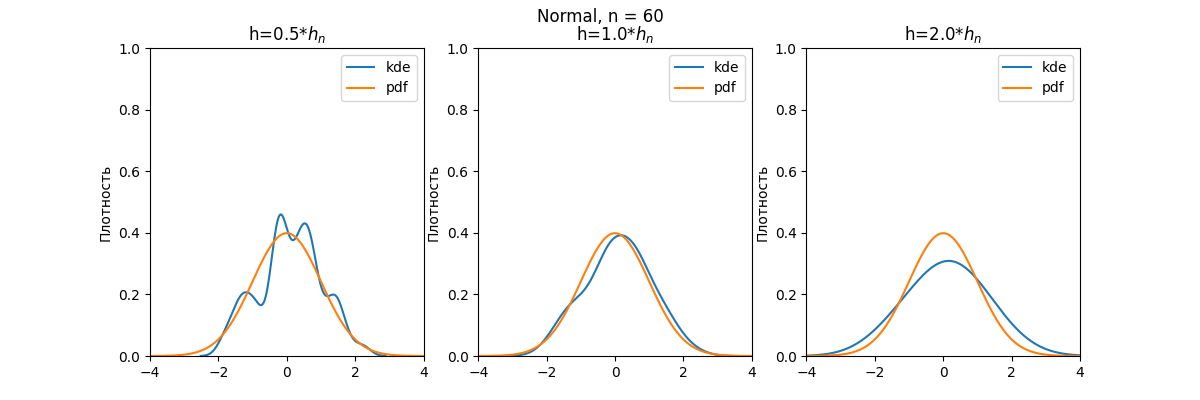
\includegraphics[width=0.8\paperwidth ]{images/kde/Normal_60.png}
  \caption{Нормальное распределение, n = 60}
\end{figure}

\begin{figure}[ht]
  \centering
  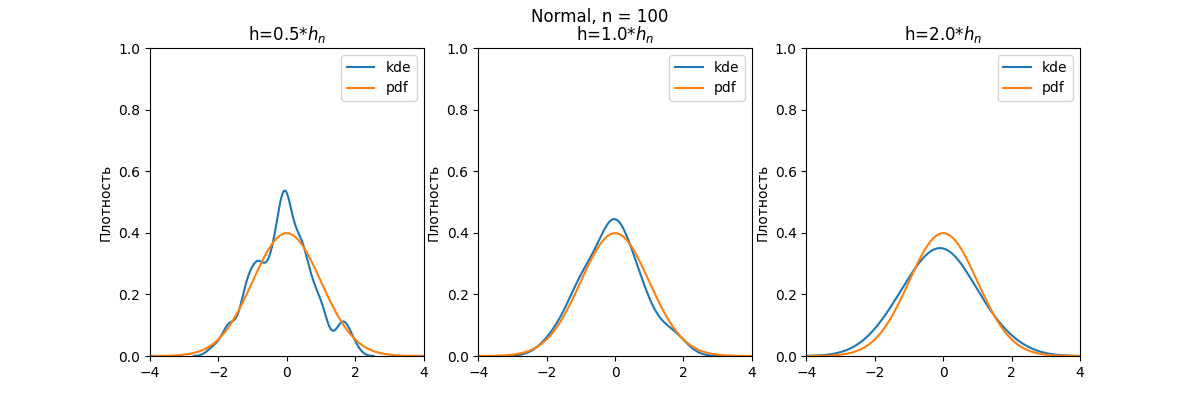
\includegraphics[width=0.8\paperwidth ]{images/kde/Normal_100.png}
  \caption{Равномерное распределение, n = 100}
\end{figure}

\begin{figure}
  \centering
  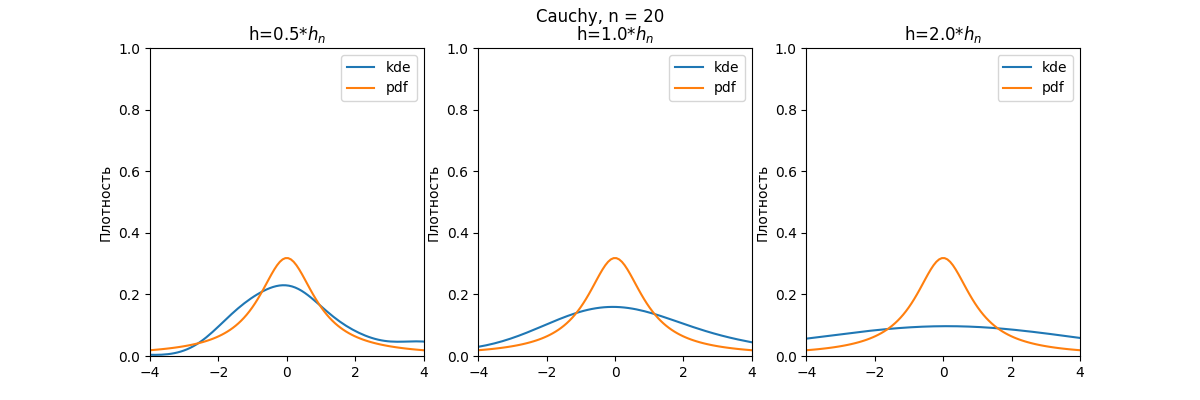
\includegraphics[width=0.8\paperwidth ]{images/kde/Cauchy_20.png}
  \caption{Распределение Коши, n = 20}
\end{figure}

\begin{figure}
  \centering
  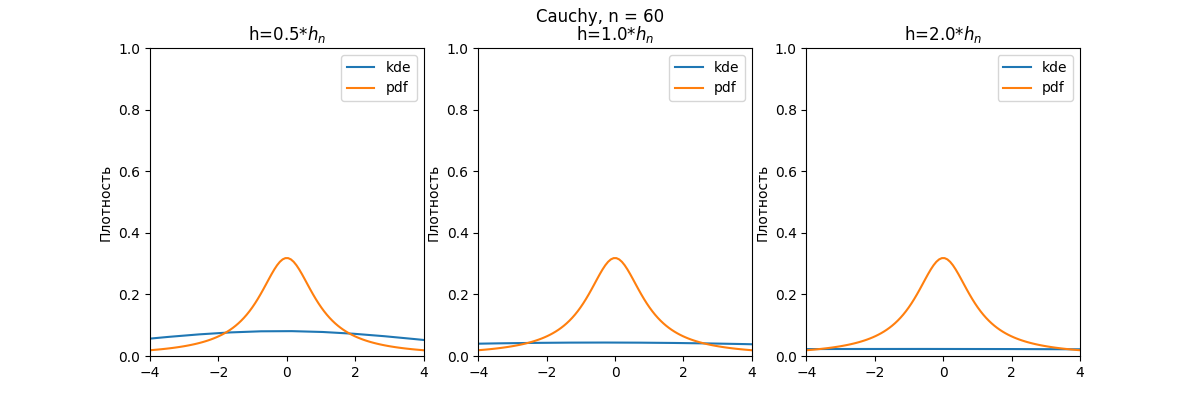
\includegraphics[width=0.8\paperwidth ]{images/kde/Cauchy_60.png}
  \caption{Распределение Коши, n = 60}
\end{figure}

\begin{figure}
  \centering
  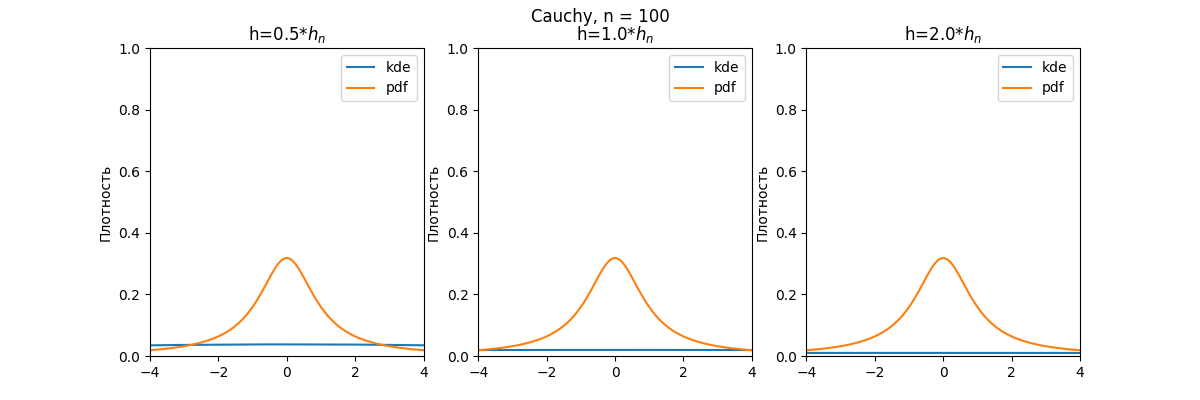
\includegraphics[width=0.8\paperwidth ]{images/kde/Cauchy_100.png}
  \caption{Распределение Коши, n = 100}
\end{figure}

\begin{figure}
  \centering
  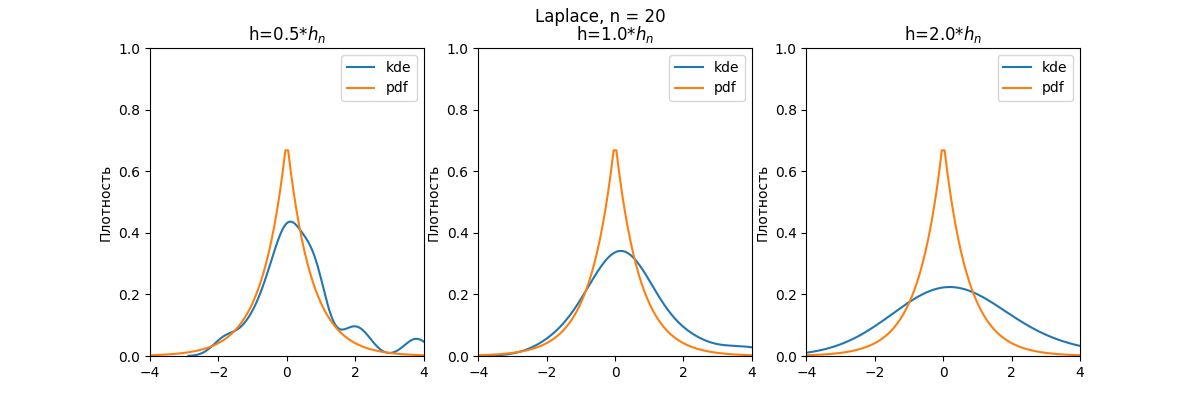
\includegraphics[width=0.8\paperwidth ]{images/kde/Laplace_20.png}
  \caption{Распределение Лапласа, n = 20}
\end{figure}

\begin{figure}
  \centering
  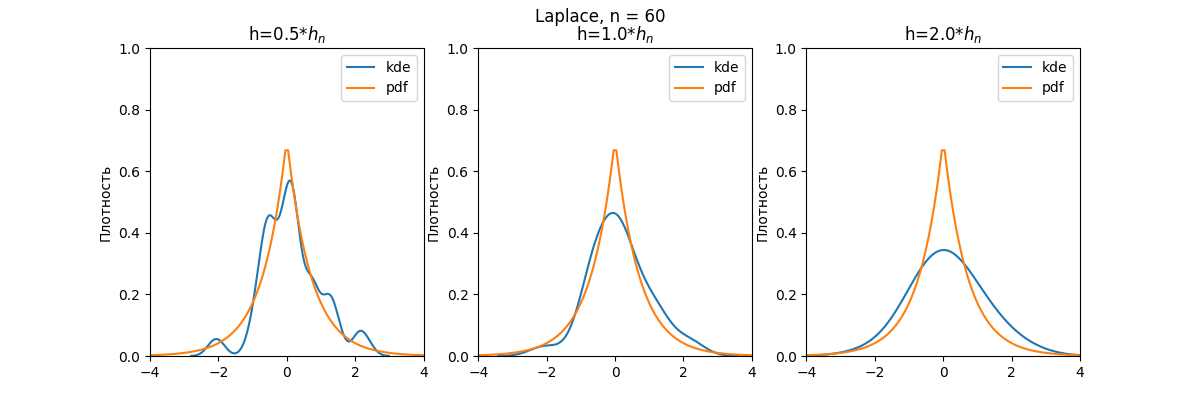
\includegraphics[width=0.8\paperwidth ]{images/kde/Laplace_60.png}
  \caption{Распределение Лапласа, n = 60}
\end{figure}

\begin{figure}
  \centering
  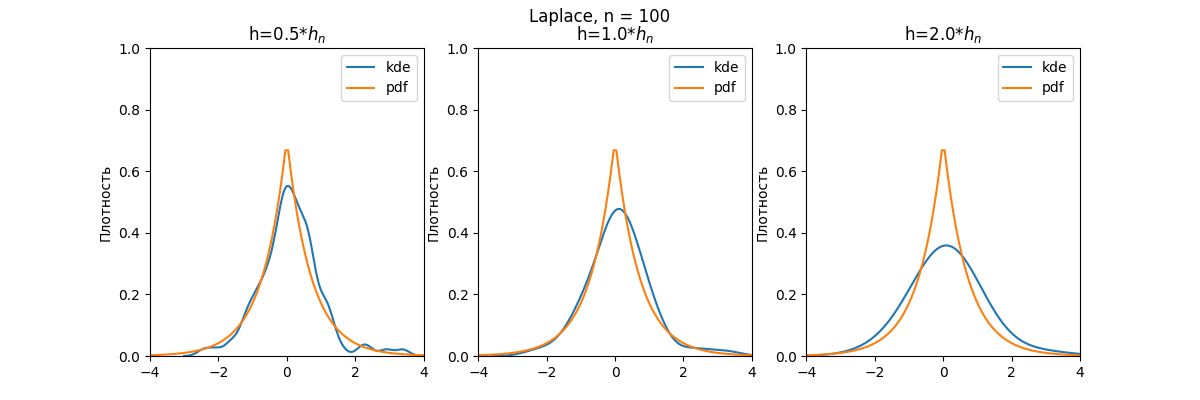
\includegraphics[width=0.8\paperwidth ]{images/kde/Laplace_100.png}
  \caption{Распределение Лапласа, n = 100}
\end{figure}

\begin{figure}
  \centering
  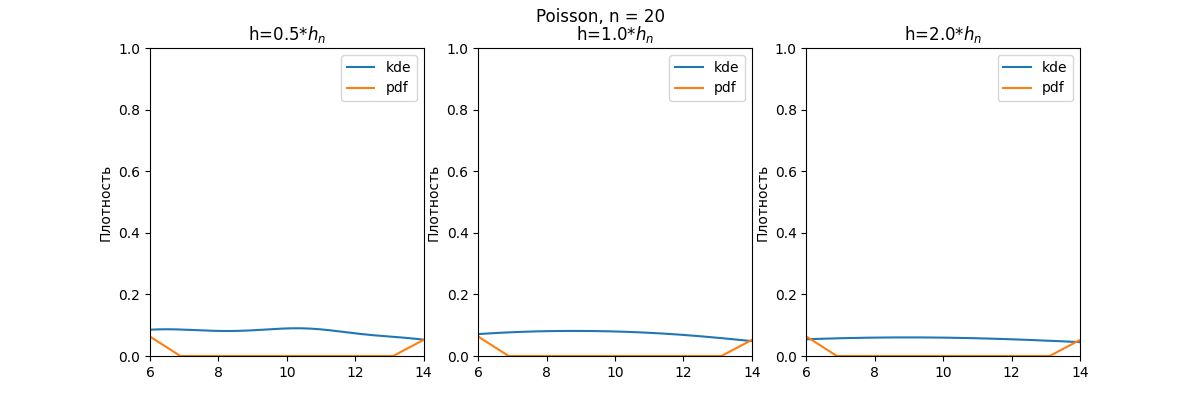
\includegraphics[width=0.8\paperwidth ]{images/kde/Poisson_20.png}
  \caption{Распределение Пуассона, n = 20}
\end{figure}

\begin{figure}
  \centering
  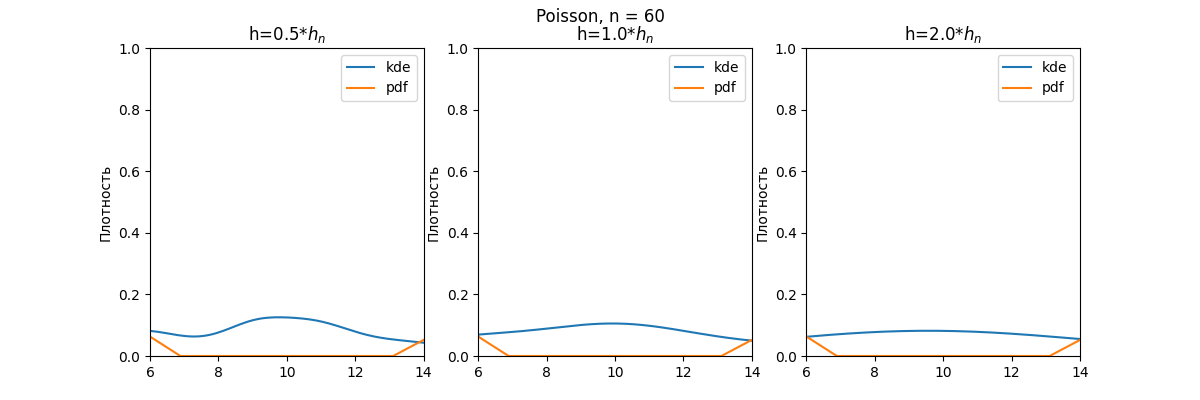
\includegraphics[width=0.8\paperwidth ]{images/kde/Poisson_60.png}
  \caption{Распределение Пуассона, n = 60}
\end{figure}

\begin{figure}
  \centering
  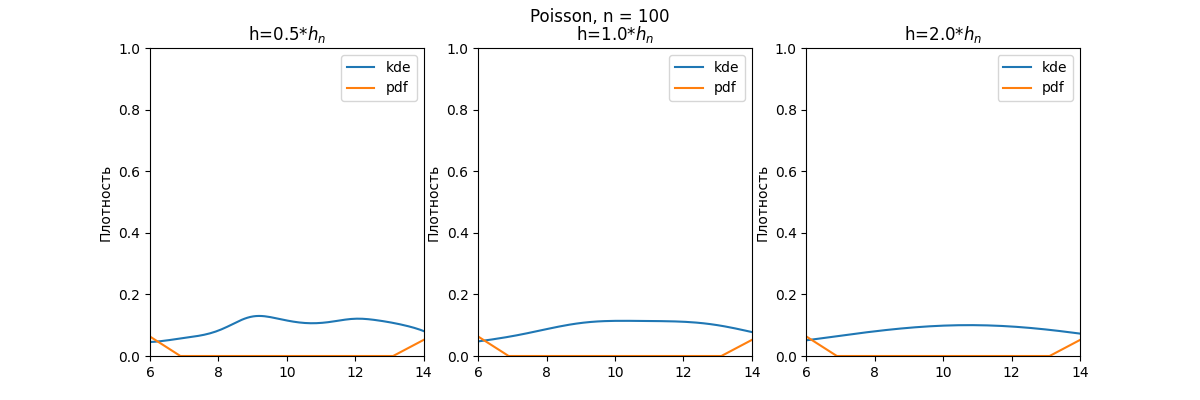
\includegraphics[width=0.8\paperwidth ]{images/kde/Poisson_100.png}
  \caption{Распределение Пуассона, n = 100}
\end{figure}

\begin{figure}
  \centering
  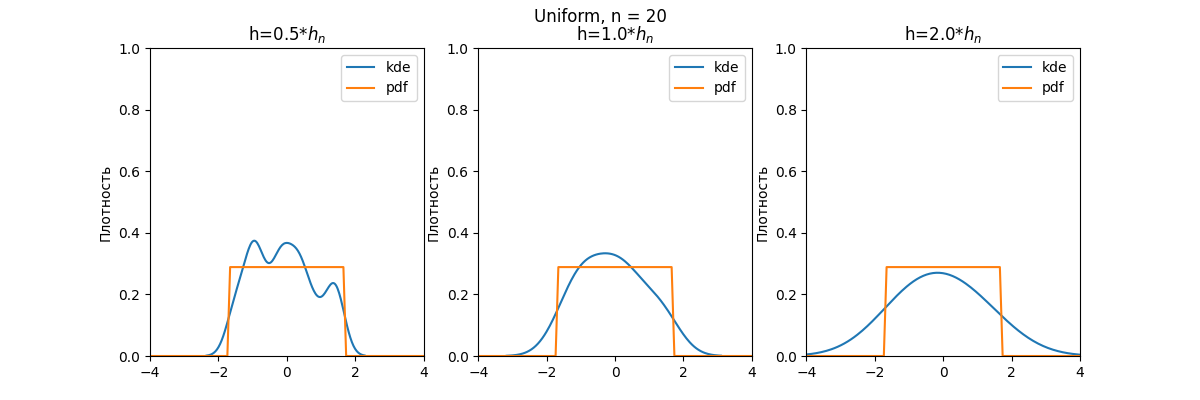
\includegraphics[width=0.8\paperwidth ]{images/kde/Uniform_20.png}
  \caption{Равномерное распределение, n = 20}
\end{figure}

\begin{figure}
  \centering
  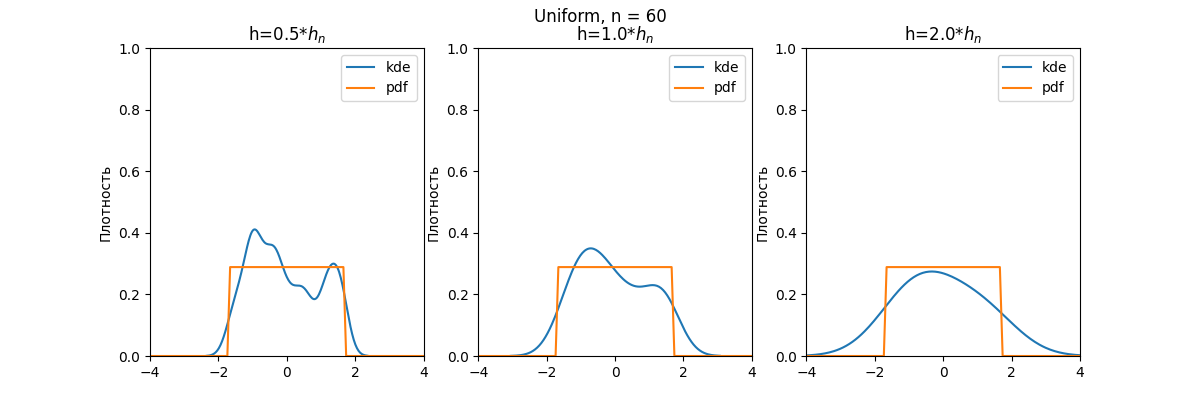
\includegraphics[width=0.8\paperwidth ]{images/kde/Uniform_60.png}
  \caption{Равномерное распределение, n = 60}
\end{figure}

\begin{figure}[!ht]
  \centering
  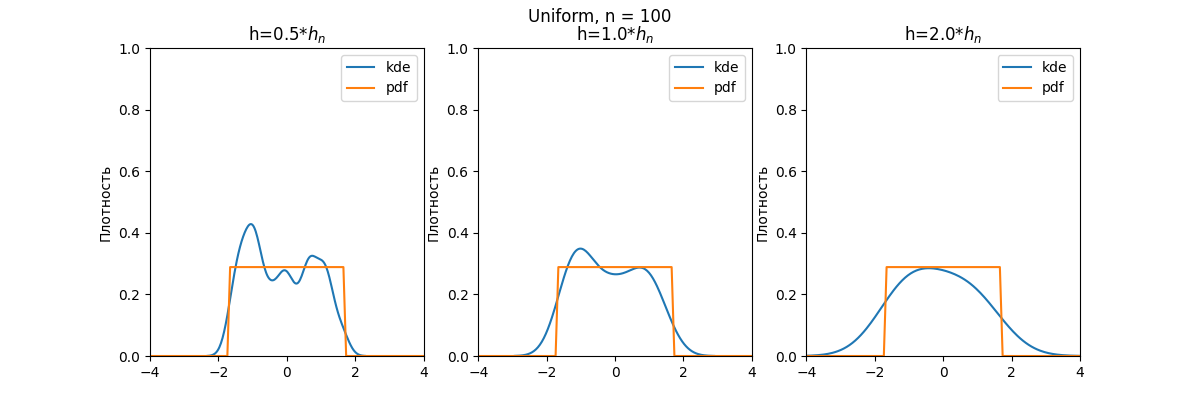
\includegraphics[width=0.8\paperwidth ]{images/kde/Uniform_100.png}
  \caption{Равномерное распределение, n = 100}
\end{figure}


\FloatBarrier
\section{Обсуждение}
\subsection{Гистограмма и график плотности вероятности}
Чем больше выборка для каждого из распределений, тем ближе
её гистограмма к графику плотности вероятности распределения. Соответственно,
чем меньше выборка, тем хуже по ней определяется характер распределения
величины.


\subsection{Характеристики положения и рассеяния}
Исходя из данных, приведенных в таблицах, можно судить о том,
что дисперсия характеристик рассеяния для распределения Коши
является некой аномалией: значения слишком большие даже при
увеличении размера выборки - понятно, что это результат выбросов, 
которые мы могли наблюдать в результатах предыдущего задания.



\subsection{Доля и теоретическая вероятность выбросов}
По данным, приведенным в таблице, можно сказать, что чем больше выборка,
тем ближе доля выбросов будет к теоретической оценке. Снова доля выбросов для
распределения Коши значительно выше, чем для остальных распределений. 
Боксплоты Тьюки действительно позволяют более наглядно и с меньшими 
усилиями оценивать важные характеристики распределений. 
Так, исходя из полученных рисунков, наглядно видно то, 
что мы довольно трудоёмко анализировали в предыдущих частях.

\subsection{Эмпирическая функция и ядерные оценки плотности распределения}
Можем наблюдать на иллюстрациях с эмпирическими функциями распределения, 
что ступенчатая эмпирическая функция распределения тем лучше приближает 
функцию распределения реальной выборки, чем мощнее эта выборка. 
Заметим так же, что для распределения Пуассона и равномерного распределения 
отклонение функций  друг от друга наибольшее.
Рисунки, посвященные ядерным оценкам, иллюстрируют сближение ядерной оценки и
функции плотности вероятности для всех $h$ с ростом размера выборки. 
Для распределения Пуассона наиболее ярко видно, как сглаживает отклонения увеличение
параметра сглаживания $h$.

В зависимости от особенностей распределений для их описания лучше подходят разные параметры
$h$ в ядерной оценке: для равномерного распределения и распределения Пуассона лучше подойдет 
параметр $h = 2h_n$, для распределения Лапласа – $h = \frac{h_n}{2}$ , а для нормального и Коши – $h = h_n$. Такие 2
значения дают вид ядерной оценки наиболее близкий к плотности, характерной данным распределениям.



\clearpage
\addcontentsline{toc}{section}{Литература}


\begin{thebibliography}{4}
    \bibitem{s:hist}
    Histogram. URL: \url{https://en.wikipedia.org/wiki/Histogram}
    \bibitem{b:probSectMath}
    Вероятностные разделы математики. Учебник для бакалавров технических направлений.//Под ред. Максимова Ю.Д. --- Спб.: «Иван Федоров», 2001. --- 592 c., илл.
    \bibitem{s:boxplot}
    Box plot. URL: \url{https://en.wikipedia.org/wiki/Box_plot}
    \bibitem{a:nonParamRegr}
    Анатольев, Станислав (2009) «Непараметрическая регрессия», Квантиль, №7, стр. 37-52.
\end{thebibliography}



\end{document}

